% Los headers de los proyectos se encuentran hardlinkeados en un directorio superior
% Es recomendable seguir esta practica para tener un header universal y que todos los
% documentos mantengan la misma estructura, y se puedan usar las mismas funciones.
%
% Para hacer un hardlink en estas carpetas hacer lo siguiente.
% Guardar todos los proyectos en una carpeta comun, como por ejemplo /home/usuario/4r1
% Clonar las repos dentro de ese directorio, eg.
%     cd /home/usuario/4r1; git clone https://path.al.link/de/la/repo
% luego copiamos uno de los header.tex al directorio superior, ej.
%     cp /home/usuario/4r1/Electronica-Aplicada-2/header.tex /home/usuario/4r1/header.tex
% Luego borramos todos los header.tex individuales (excluyendo el del directorio 4r1)
%     cd /home/usuario/4r1; for x in $(ls | grep -v header.tex); do rm $x/header.tex; done
% Como ultimo paso linkeamos los headers con un hard link.
%     cd /home/usuario/4r1; for x in $(ls | grep -v header.tex); do ln header.tex $x/header.tex; done
%
% IMPORTANTE, debe ser un hardlink,y no uno simbolico como se acostumbra,ya que los sistemas 
% de revisionado de archivos como github tratan a los links simbolicos como tales, y no 
% almacenan el contenido del archivo.
%
% Tambien se obvio, la idea luego de esto, es que al modificar cualquier header, se modifican el resto
% El proceso completo para hacer los pasos anteriores se encuentra en el siguiente script:
% https://gist.github.com/RNacho/e4c1ac3fdafc2045356cc92c7f966d54
%

\documentclass[tikz,11pt, a4paper]{report}
\setcounter{secnumdepth}{1}
\setcounter{tocdepth}{2}
\usepackage[margin=1.0in]{geometry}

\usepackage[spanish]{layout}
\usepackage[activeacute,spanish]{babel}
\usepackage[utf8]{inputenc}
\usepackage[]{subfig}
\usepackage[colorlinks]{hyperref}
\usepackage{import} %reemplaza a input, incluyendo el path relativo al archivo
\usepackage{lipsum}

\usepackage[siunitx,american]{circuitikz}
\usepackage{tikz}
\usetikzlibrary{arrows}
\usetikzlibrary{shapes}
\usetikzlibrary{calc}

\usepackage{pgfplots}

\usepackage{textcomp}

\usepackage{commath}
\usepackage{amsmath}
\usepackage{amssymb}
\usepackage{mathtools}
\usepackage[makeroom]{cancel}
\usepackage{xfrac}
\usepackage{adjustbox}

\usepackage{tabu}
\usepackage{multirow}
\usepackage{tabularx}


\newcommand{\rotarTester}[2]
{  % #1 = name , #2 = rotation angle
\begin{scope}[transform shape,rotate=#2]
\draw[thick] (#1)node(){$\mathbf V$} circle (11pt);
\draw[rotate=45,-latex] (#1)  +(-17pt,0) --+(17pt,0);
\end{scope}
}

\usepackage{fancyhdr}

\lhead[]{}
\chead[]{}
\rhead[]{}
\renewcommand{\headrulewidth}{0pt}

\lfoot[UTN-FRC]{UTN FRC}
\cfoot[\thepage]{\thepage}
\rfoot[Gabriel González - 4R1 - G1]{Gabriel González - 4R1 - G1}
\renewcommand{\footrulewidth}{0.5pt}

\fancypagestyle{plain}{
\fancyhead[]{}
\fancyhead[]{}
\fancyhead[]{}
\fancyfoot[UTN-FRC]{UTN-FRC}
\fancyfoot[\thepage]{\thepage}
\fancyfoot[Gabriel González - 4R1 - G1]{Gabriel González - 4R1 - G1}
\renewcommand{\headrulewidth}{0pt}
\renewcommand{\footrulewidth}{0.5pt}
}

\pagestyle{fancy}

\begin{document}
\chapter{Amplificadores realimentados}
\section{Efectos de la realimentación negativa}
\begin{itemize}
	\item Mejora estabilidad de la ganancia. 
	\item Reducción de las señales espurias (ruidos externos e internos).
	\item Cambio en las impedancias de entrada y de salida.
	\item Aumento del ancho de banda del amplificador.
	\item Aumento de la estabilidad de frecuencia.
\end{itemize}
\section{Amplificador de tensión con muestra de tensión en serie}

\begin{figure}[h!]
	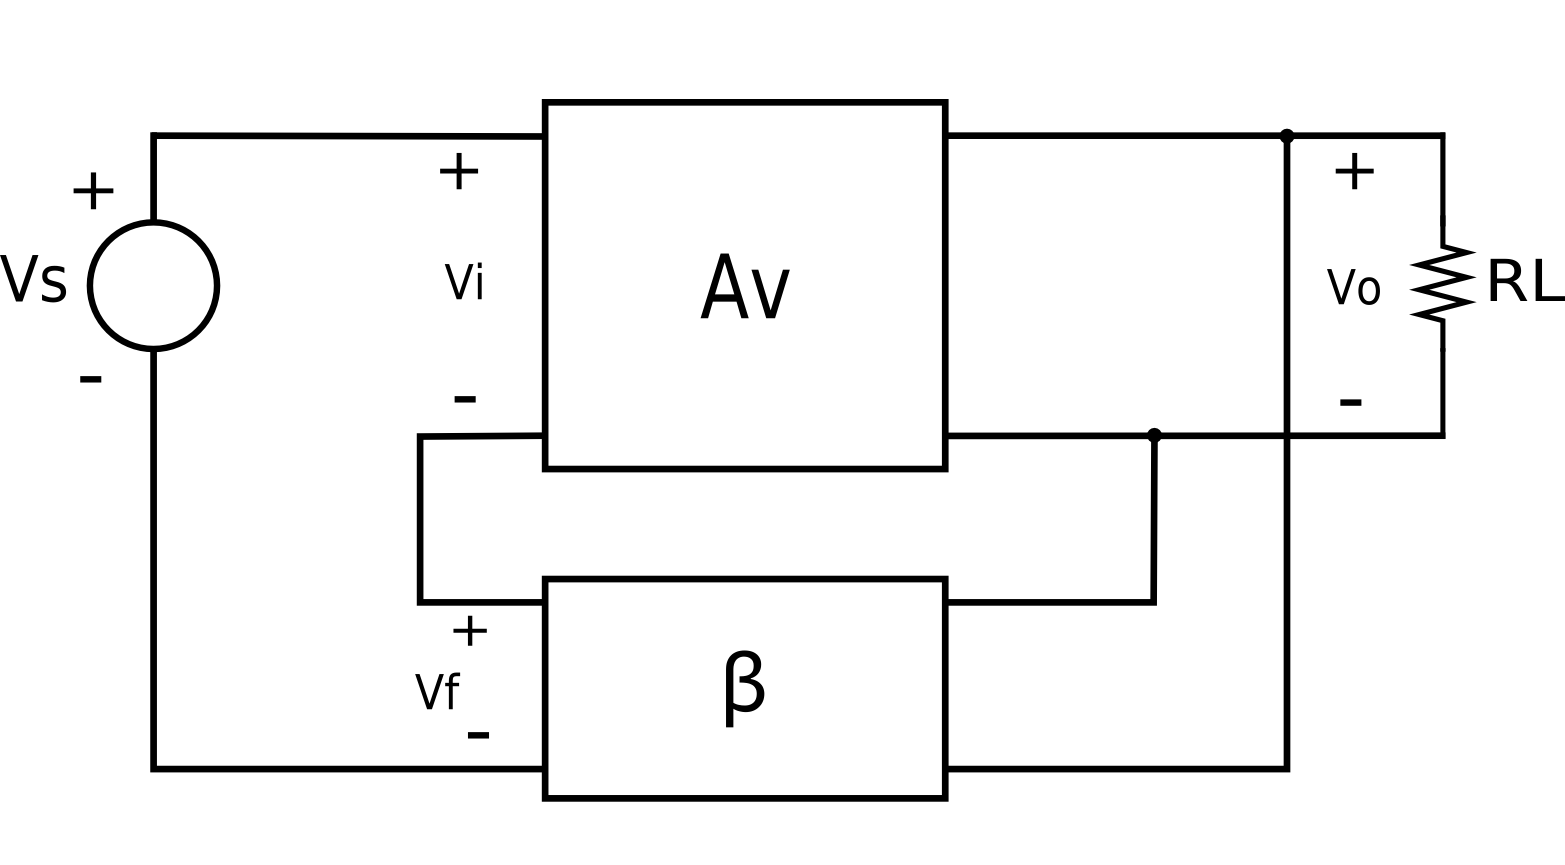
\includegraphics[width=0.8\linewidth]{./img/1.png}
	\centering
	\caption{Esquema general de bloques de un amplificador de tensión con muestra de tensión en serie}
	\label{fig:amp1}
\end{figure}


\section{Amplificador de transconductancia con muestra de corriente en serie}

\begin{figure}[h!]
	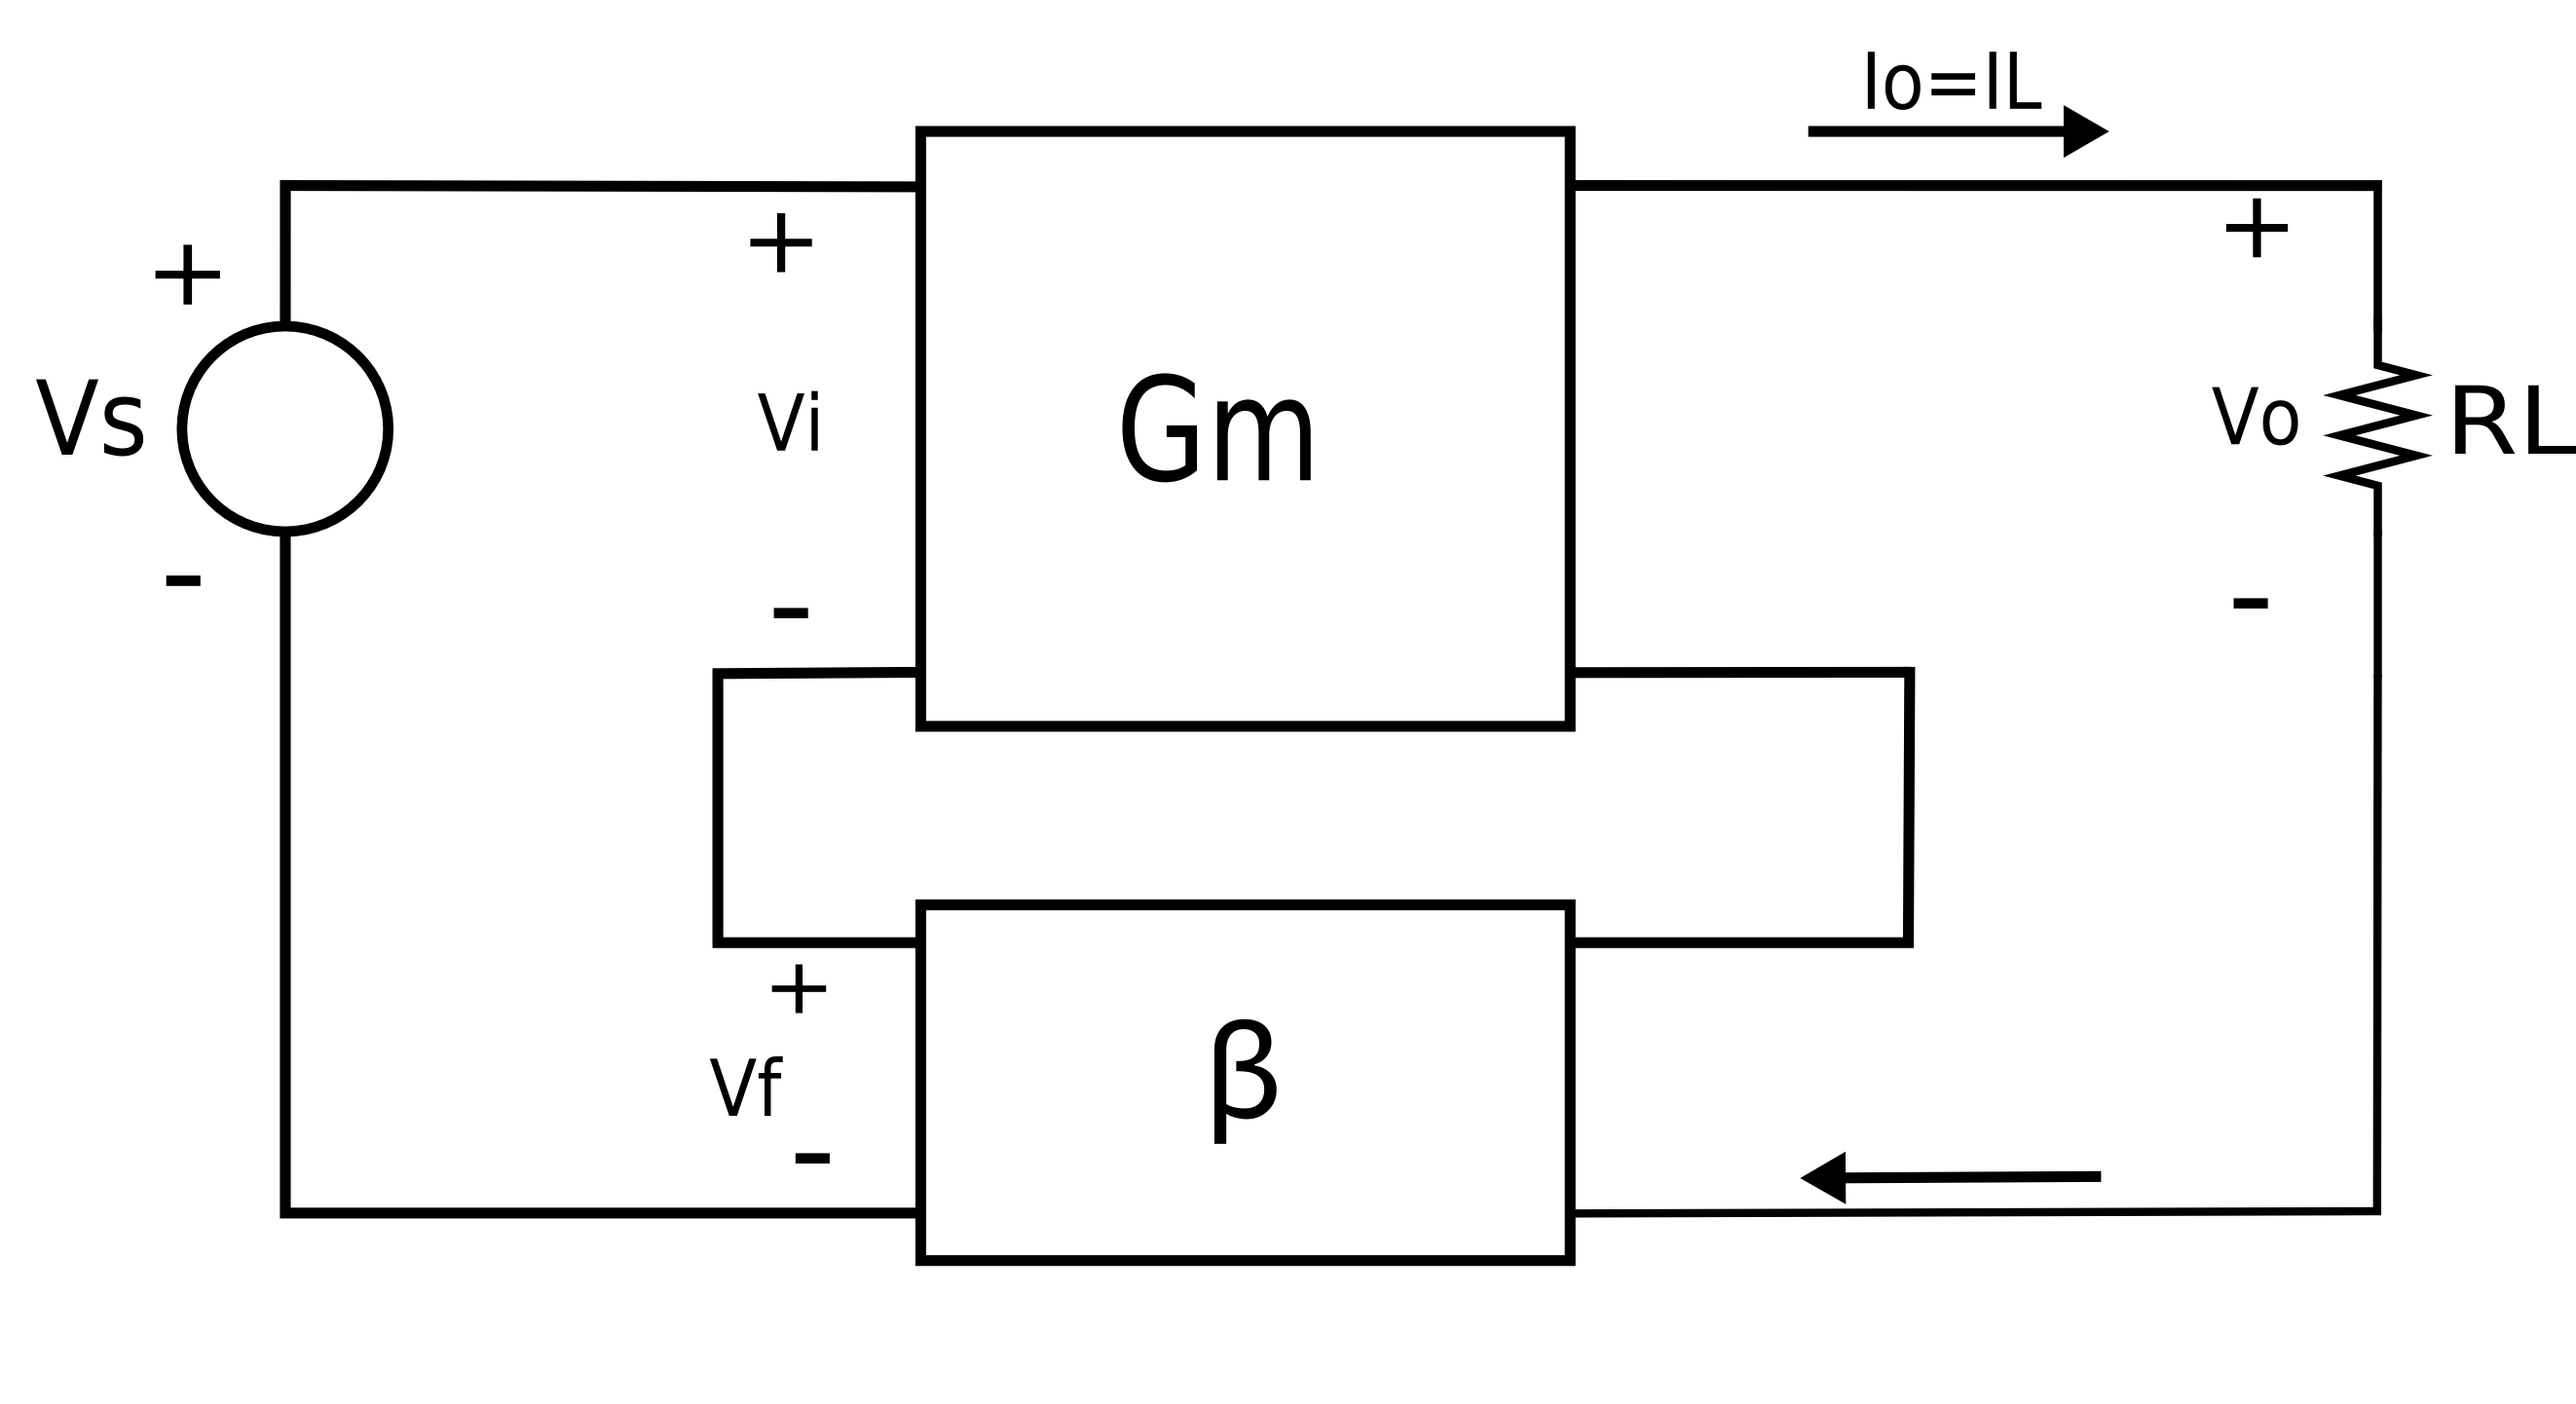
\includegraphics[width=0.8\linewidth]{./img/2.png}
	\centering
	\caption{Esquema general de bloques de un amplificador de transconductancia con muestra de corriente en serie}
	\label{fig:amp2}
\end{figure}

\newpage
\section{Amplificador de corriente con muestra de corriente en paralelo}

\begin{figure}[h!]
	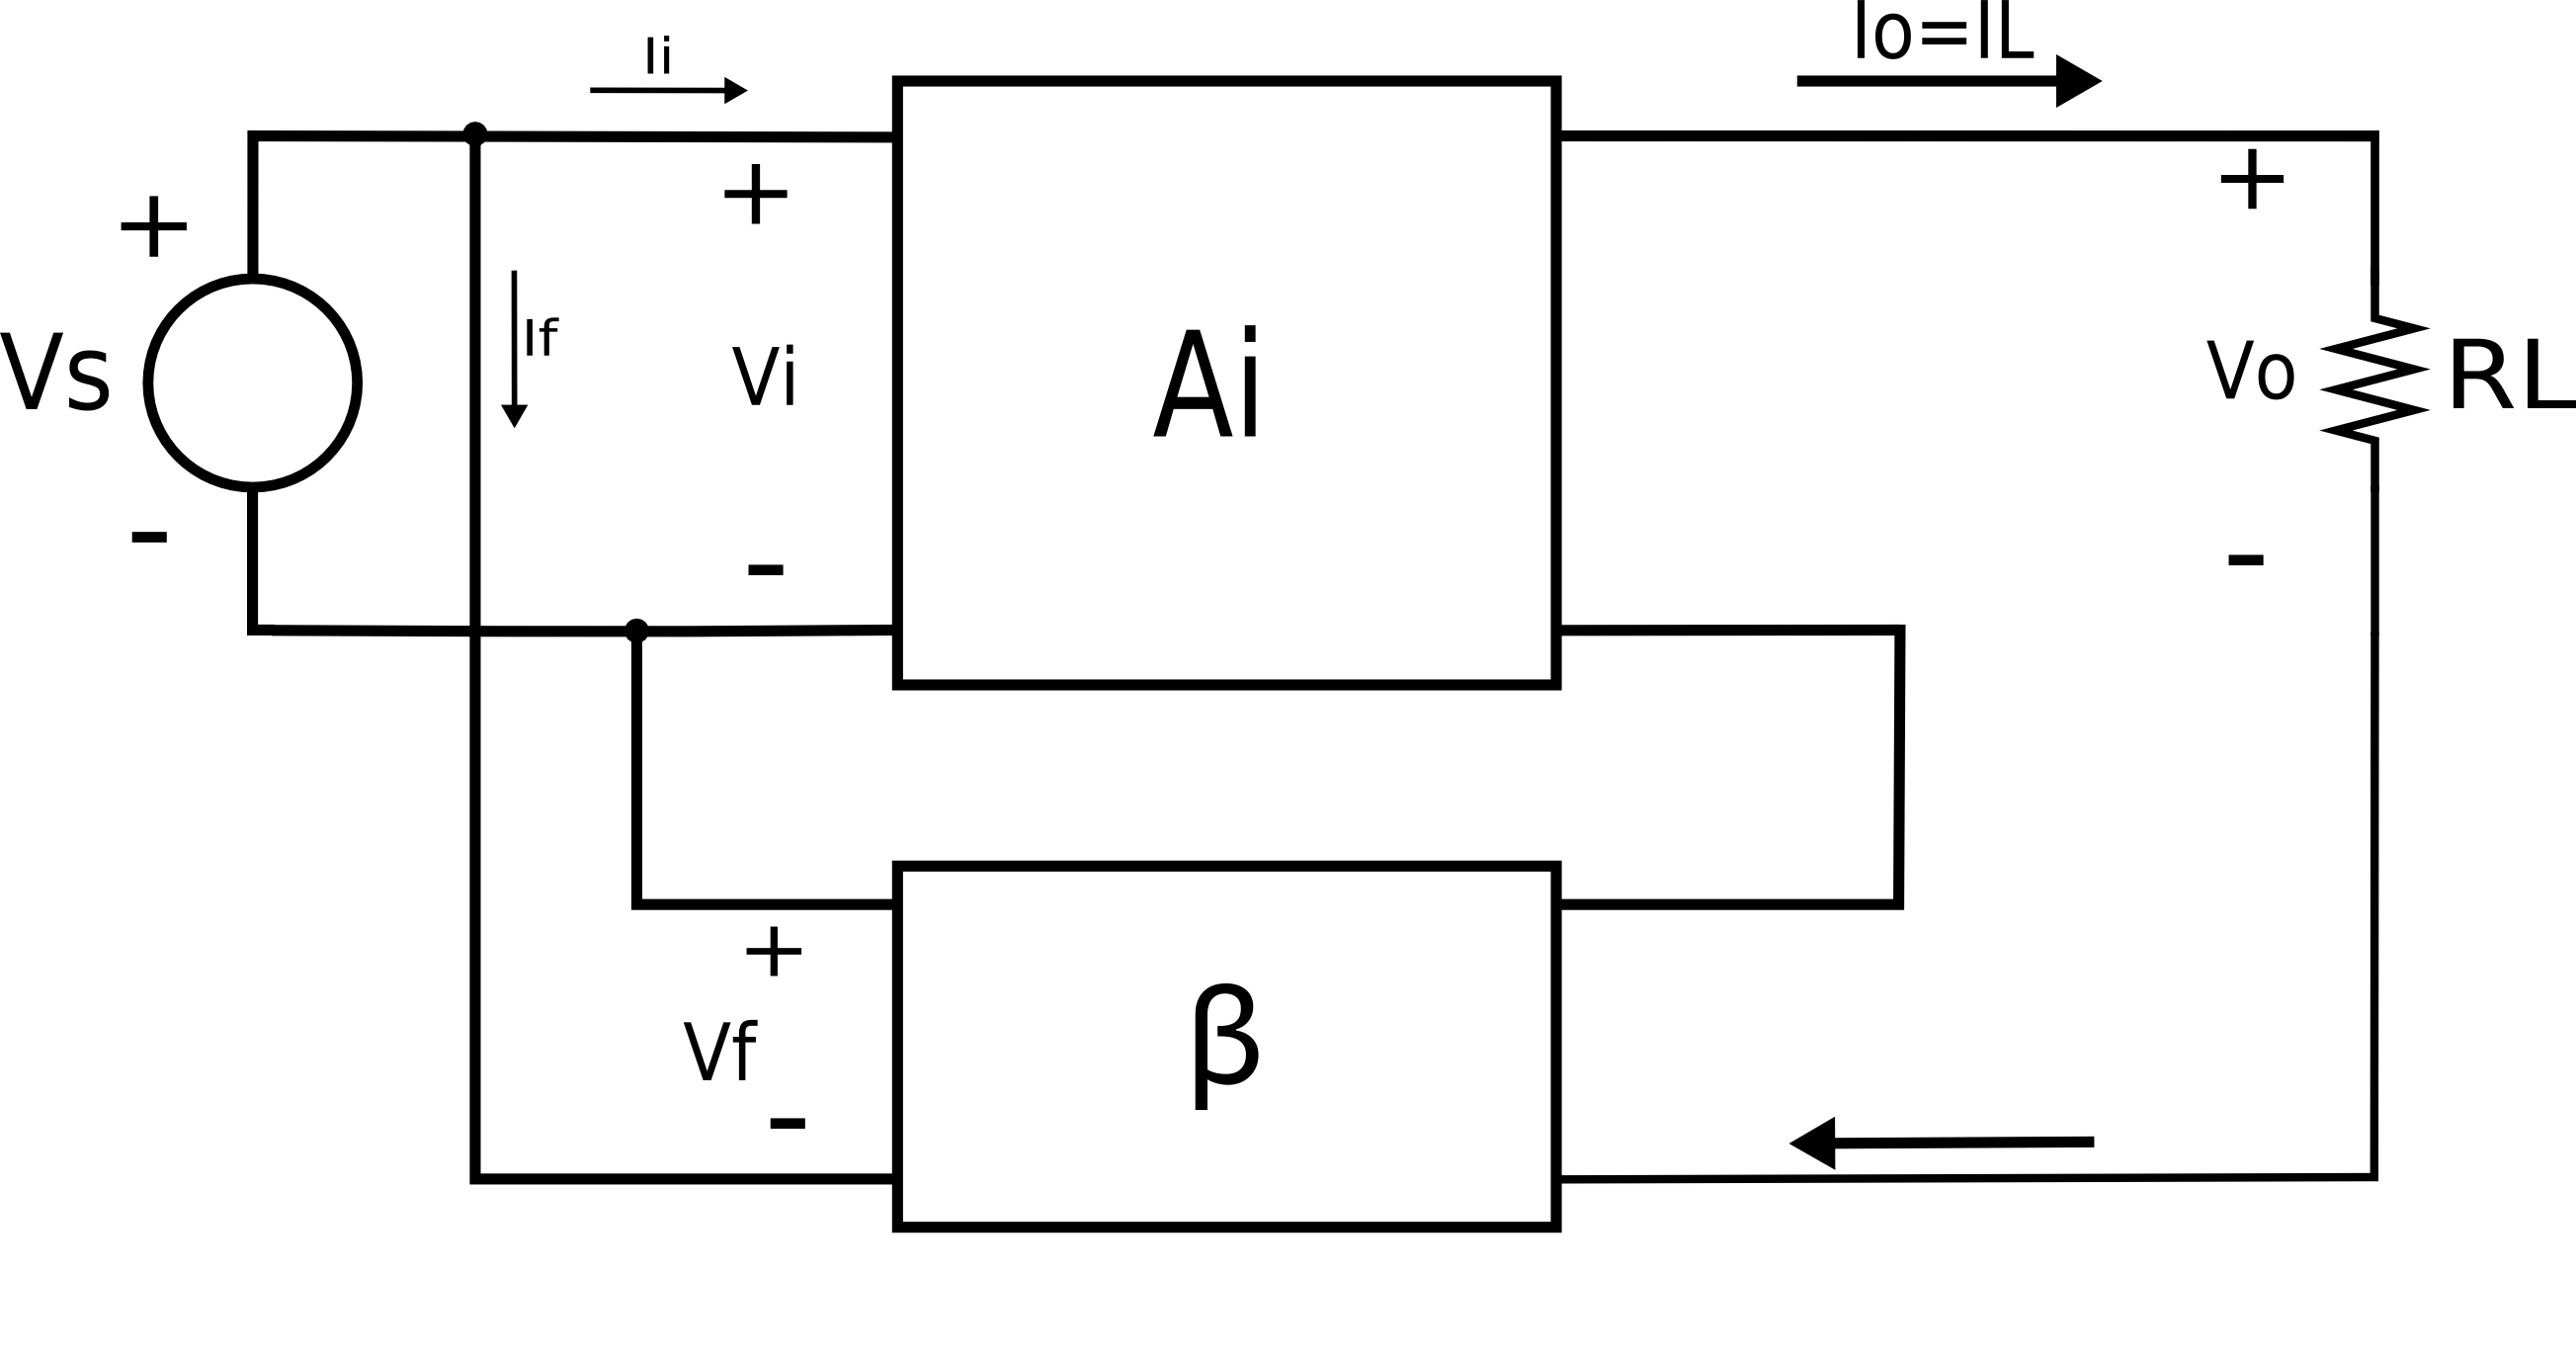
\includegraphics[width=0.8\linewidth]{./img/3.png}
	\centering
	\caption{Esquema general de bloques de un amplificador de corriente con muestra de corriente en paralelo}
	\label{fig:amp3}
\end{figure}

\section{Amplificador de transresistencia con muestra de tensión en paralelo}

\begin{figure}[h!]
	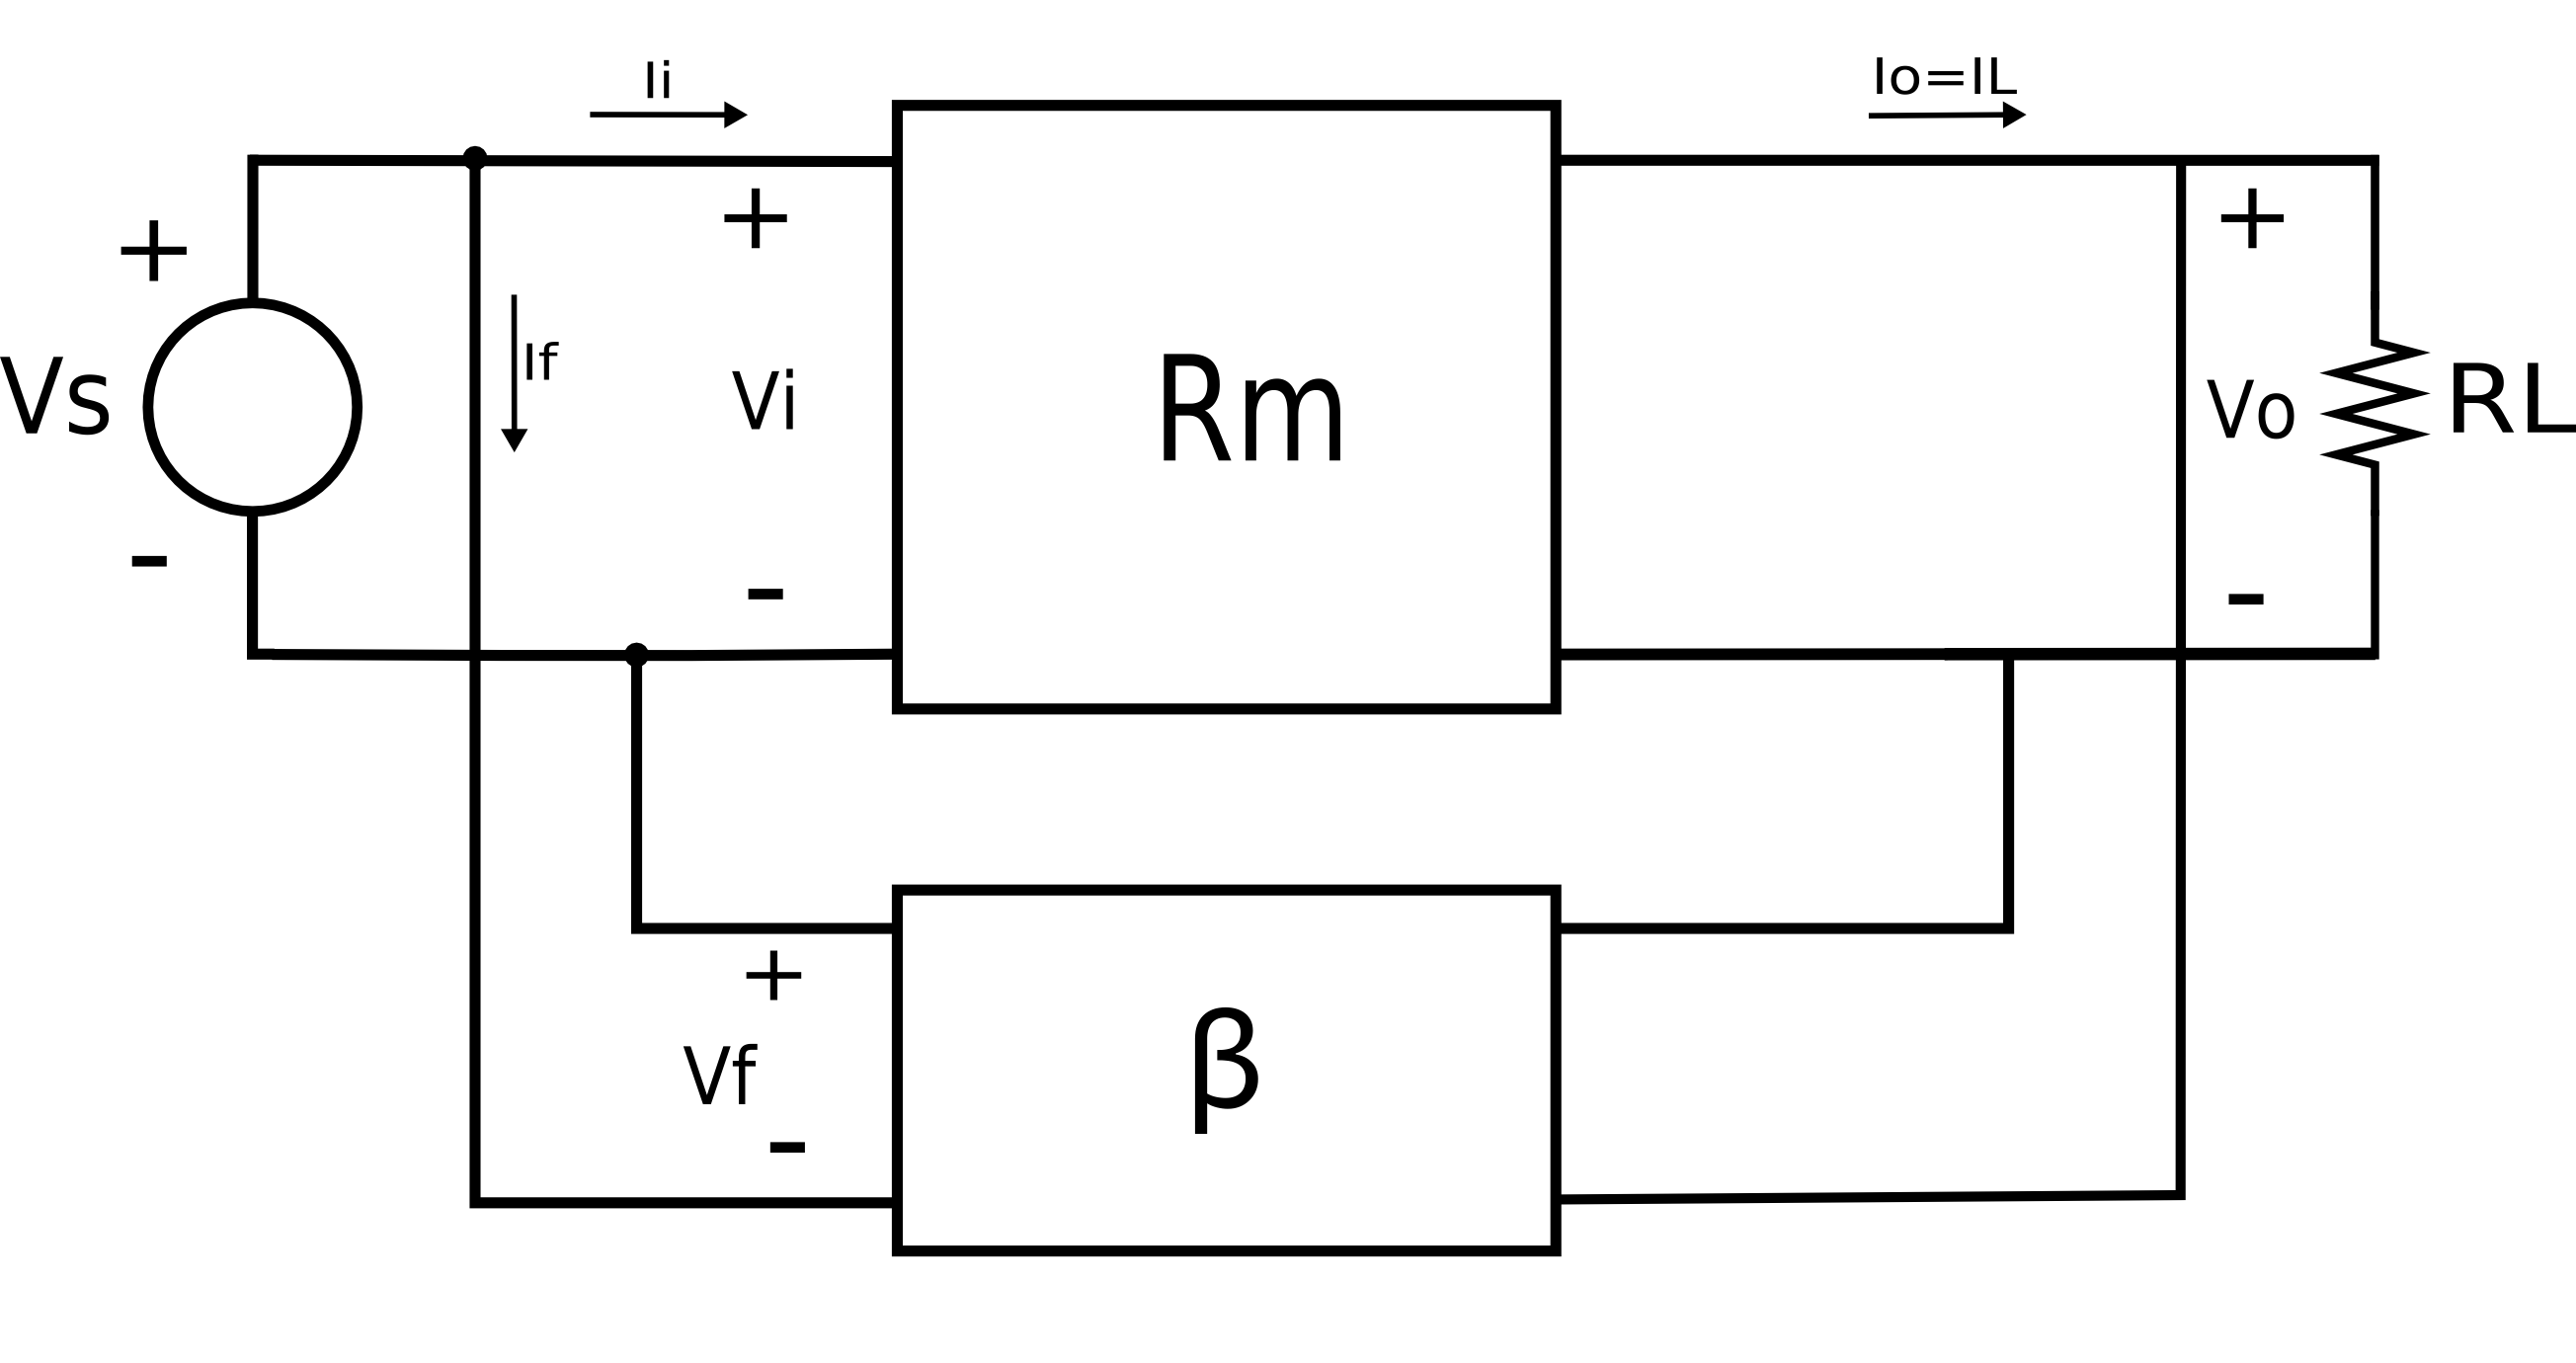
\includegraphics[width=0.8\linewidth]{./img/4.png}
	\centering
	\caption{Esquema general de bloques de un amplificador de transresistencia con muestra de tensión en paralelo}
	\label{fig:amp4}
\end{figure}

\end{document}
